% header
\documentclass[10pt,a4paper]{article}

\usepackage[utf8]{inputenc}
\usepackage{hyperref}
\usepackage{amssymb}
\usepackage{amsmath}
\usepackage{listings}
\usepackage{graphicx}

% the document
\begin{document}

\title{Worksheet $1$\\
\small{Practical Lab Numerical Computing}}
\author{Andrii Lischishin \and Lars Schleithoff \and Hendrik Kleikamp}
\date{\today}
\maketitle

\section*{Task 1}

The code generates two uniformly distributed random numbers on the interval $[0,1]$. The first random number is generated by a standard $C++$ function called $rand$.
The second random number is generated by a generator from the gsl library.
The difference lies in the generator used for creating those random numbers. The second way uses a \texttt{gsl\_rng} pointer which transports the information on the selected generator. 
One can use the same pointer for differently distributed random numbers, e.g. \texttt{double gsl\_ran\_gaussian (const gsl\_rng * r, double sigma)}, where $\mu=0$. 

If you remove the expression (double), the result will be $0$ due to rounding to the next smaller integer. The rand function creates an integer and \texttt{RAND\_MAX} is a constant integer as well. 

In fact, there won't be any different random numbers each time you run the code snippet, because there is no seed declared. 

\section*{Task 2}

\begin{center}
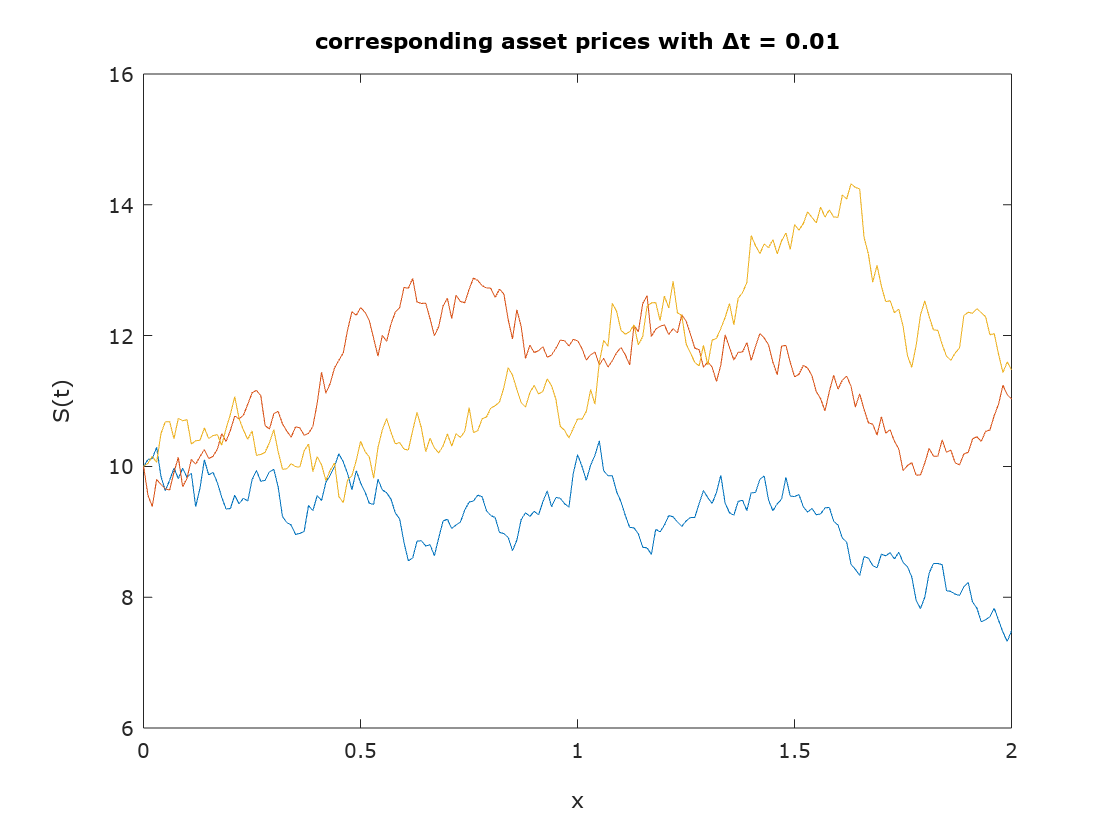
\includegraphics[scale=0.5]{asset_001.jpeg}		
\end{center}	

\begin{center}
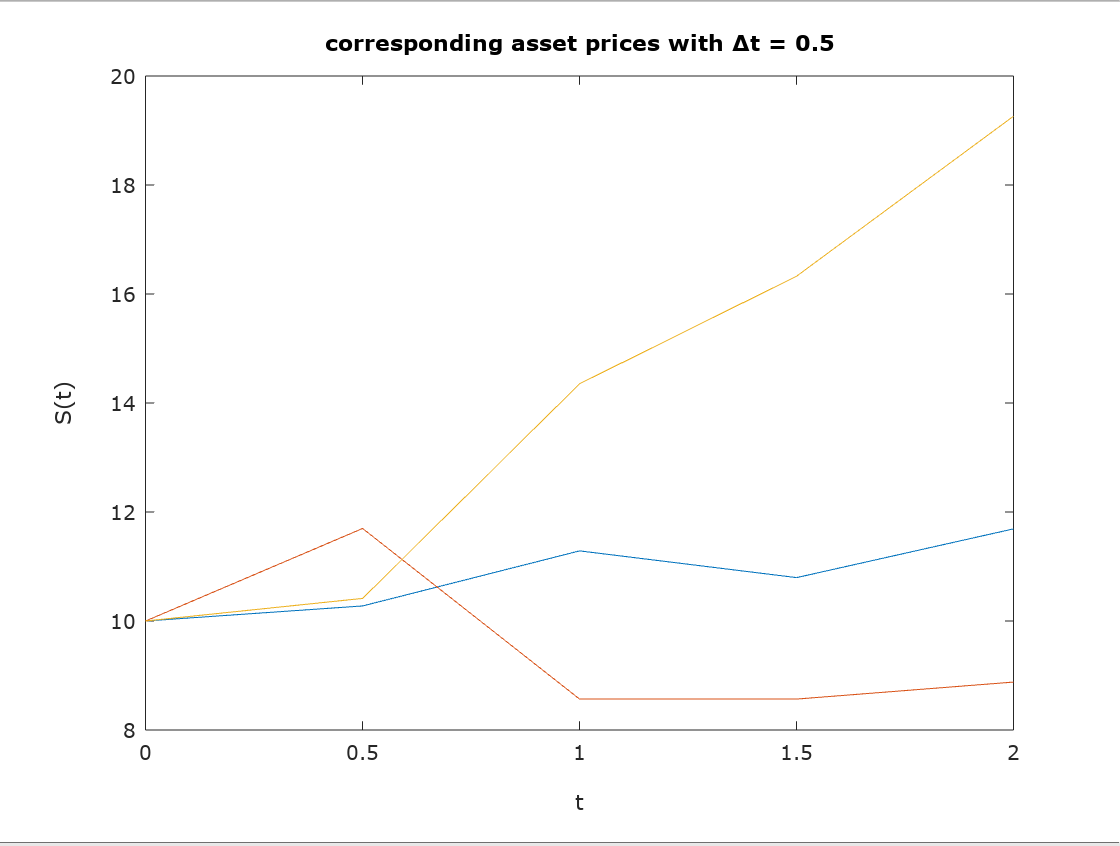
\includegraphics[scale=0.5]{asset_05.jpeg}		
\end{center}	

\section*{Task 3}

The MATLAB script divides the interval $[0,1]$ into $100$ equidistant sections. The number of random values in each interval is then depicted by the density value of the points in the plot.

Fig.1 shows what happens if the interval bounds in step $1$ of the rejection sampling algorithm are chosen to small, e.g. $[-2,2]$.  


\section*{Task 4}

Let $X$ be an uniformly distributed random variable on $(0,1)$, and $\Phi(t)=\frac{1}{\sqrt{2 \pi}}\int_{-\infty}^{t}e^{-\frac{x^2}{2}}dx$.
 
$\Phi(t)$ is continuous and monotically increasing, therefore the solution of $\Phi(t)=y$, which is $\frac{1}{\sqrt{2 \pi}}\int_{-\infty}^{t}e^{-\frac{x^2}{2}}dx=y$, is unique. Now, the inverse function $f:(0,1)\rightarrow \mathbb{R}$ takes in a value from the interval $(0,1)$ and the output is in $\mathbb{R}$.

Specifically, $\Phi(t)=\frac{1}{\sqrt{2 \pi}}\int_{a}^{b}e^{-\frac{x^2}{2}}dx=\Phi(b)-\Phi(a)$. This implies that $a\leq f(X) \leq b \Leftrightarrow \Phi(a)\leq X \leq \Phi(b)$, since $\Phi(f(X))=X$.

For this reason, applying the inverse function of the standard normal distribution to an uniformly distributed random variable leads to a standard normal distributed random variable.  

\section*{Task 5}

The basic idea is to approximate the integral on different intervals by different functions. The first if-clause uses the symmetry of the standard normal distribution and the fact that 
\[
	\frac{1}{\sqrt{2 \pi}}\int\limits_{-\infty}^{\infty}e^{-\frac{x^2}{2}}dx=1.
\]

For $x\geq 6$, the accuracy of $8$ digits has already been reached, so the algorithm returns the value $1$.

\section*{Task 6}

\begin{center}
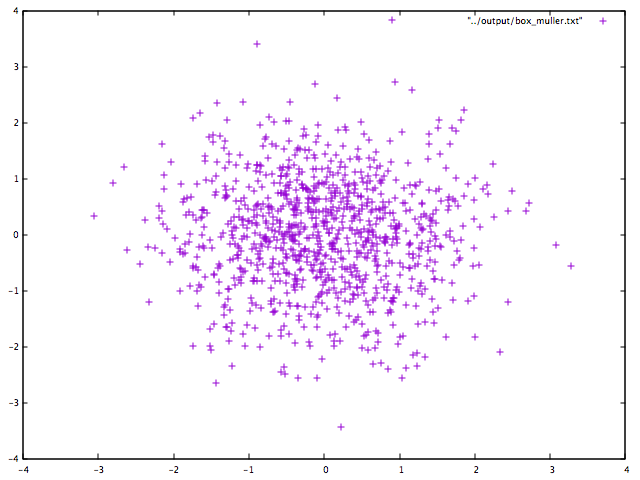
\includegraphics[scale=0.4]{box_mueller.jpeg}
\end{center}

\section*{Task 7}

By transformation to polar coordinates, it follows that
\begin{align*}
	z_1=r cos(\phi), z_2=r sin(\phi)
\end{align*}   

with $r=\sqrt{-2ln(u_1)}, \phi=2\pi u_2$. 

$\phi\in (0,2\pi)$ is uniformly distributed on circles, and the square of the radius of these circles, $r^2=Z_1^2+Z_2^2$, has Chi-squared distribution.

The product of those two random variables ist normally distributed:
\begin{align*}
\frac{1}{2}e^{-\frac{1}{2}r^2}d(r^2)d\phi = \frac{1}{2\pi}e^{-\frac{1}{2}r^2}rdrd\phi = \frac{1}{2\pi}e^{-\frac{1}{2}(z_1^2+z_2^2)}dz_1dz_2
\end{align*} 

Therefore, $z_1$ and $z_2$ are standard normally distributed.

\section*{Task 8}

The main advantage of the algorithm stated on the sheet is that $\hat{\mu}$ doesn't need to be calculated seperately, for this reason only one for-loop is needed. Furthermore, cancellation can be avoided.

$\alpha, \beta$ and $\sigma$ can be expressed in the following way ($k$ is the number of the iteration of the forloop):

\begin{gather*}
\alpha_k = \frac{\sum_{i=1}^k x_i}{k} \\
\beta_k = \beta_{k-1}+\frac{k}{k+1}\bigg(x_k-\bigg(\frac{x_1+x_2+...+x_{k}}{k}\bigg)\bigg)^2 \\
\sigma^2 = \frac{1}{N-1}\sum_{k=1}^N\beta_k
\end{gather*}

For $k \to \infty$, $\beta_k$ converges to $\sum_{k=1}^N (x_k-\hat{\mu})^2$:

\begin{gather*}
\underbrace{\frac{k}{k+1}}_{\to 1}\bigg(x_k-\bigg(\underbrace{\frac{x_1+x_2+...+x_{k}}{k+1}}_{\to \hat{\mu}}\bigg)\bigg)^2 \underrightarrow{k\to\infty} (x_k-\hat{\mu})^2 \\
\beta = \sum_{k=1}^N \beta_k \to \sum_{k=1}^N (x_k-\hat{\mu})^2 \\
\sigma^2 = \frac{1}{N-1}\sum_{k=1}^N\beta_k \to \frac{1}{N-1} \sum_{i=1}^N (x_k-\hat{\mu})^2 \\
\end{gather*}

For this reason, the algorithm converges to the variance of $(x_i)_{i=1}^N$.

\section*{Task 9}

The plot illustrates, how for small $N$, the deviation from the correct result is high and how it then converges to $\sigma$ for higher $N$. This matches with the behaviour of the algorithm, which might have a great inaccuracy for small $N$, but gets more exact the bigger $N$ gets.

\begin{center}
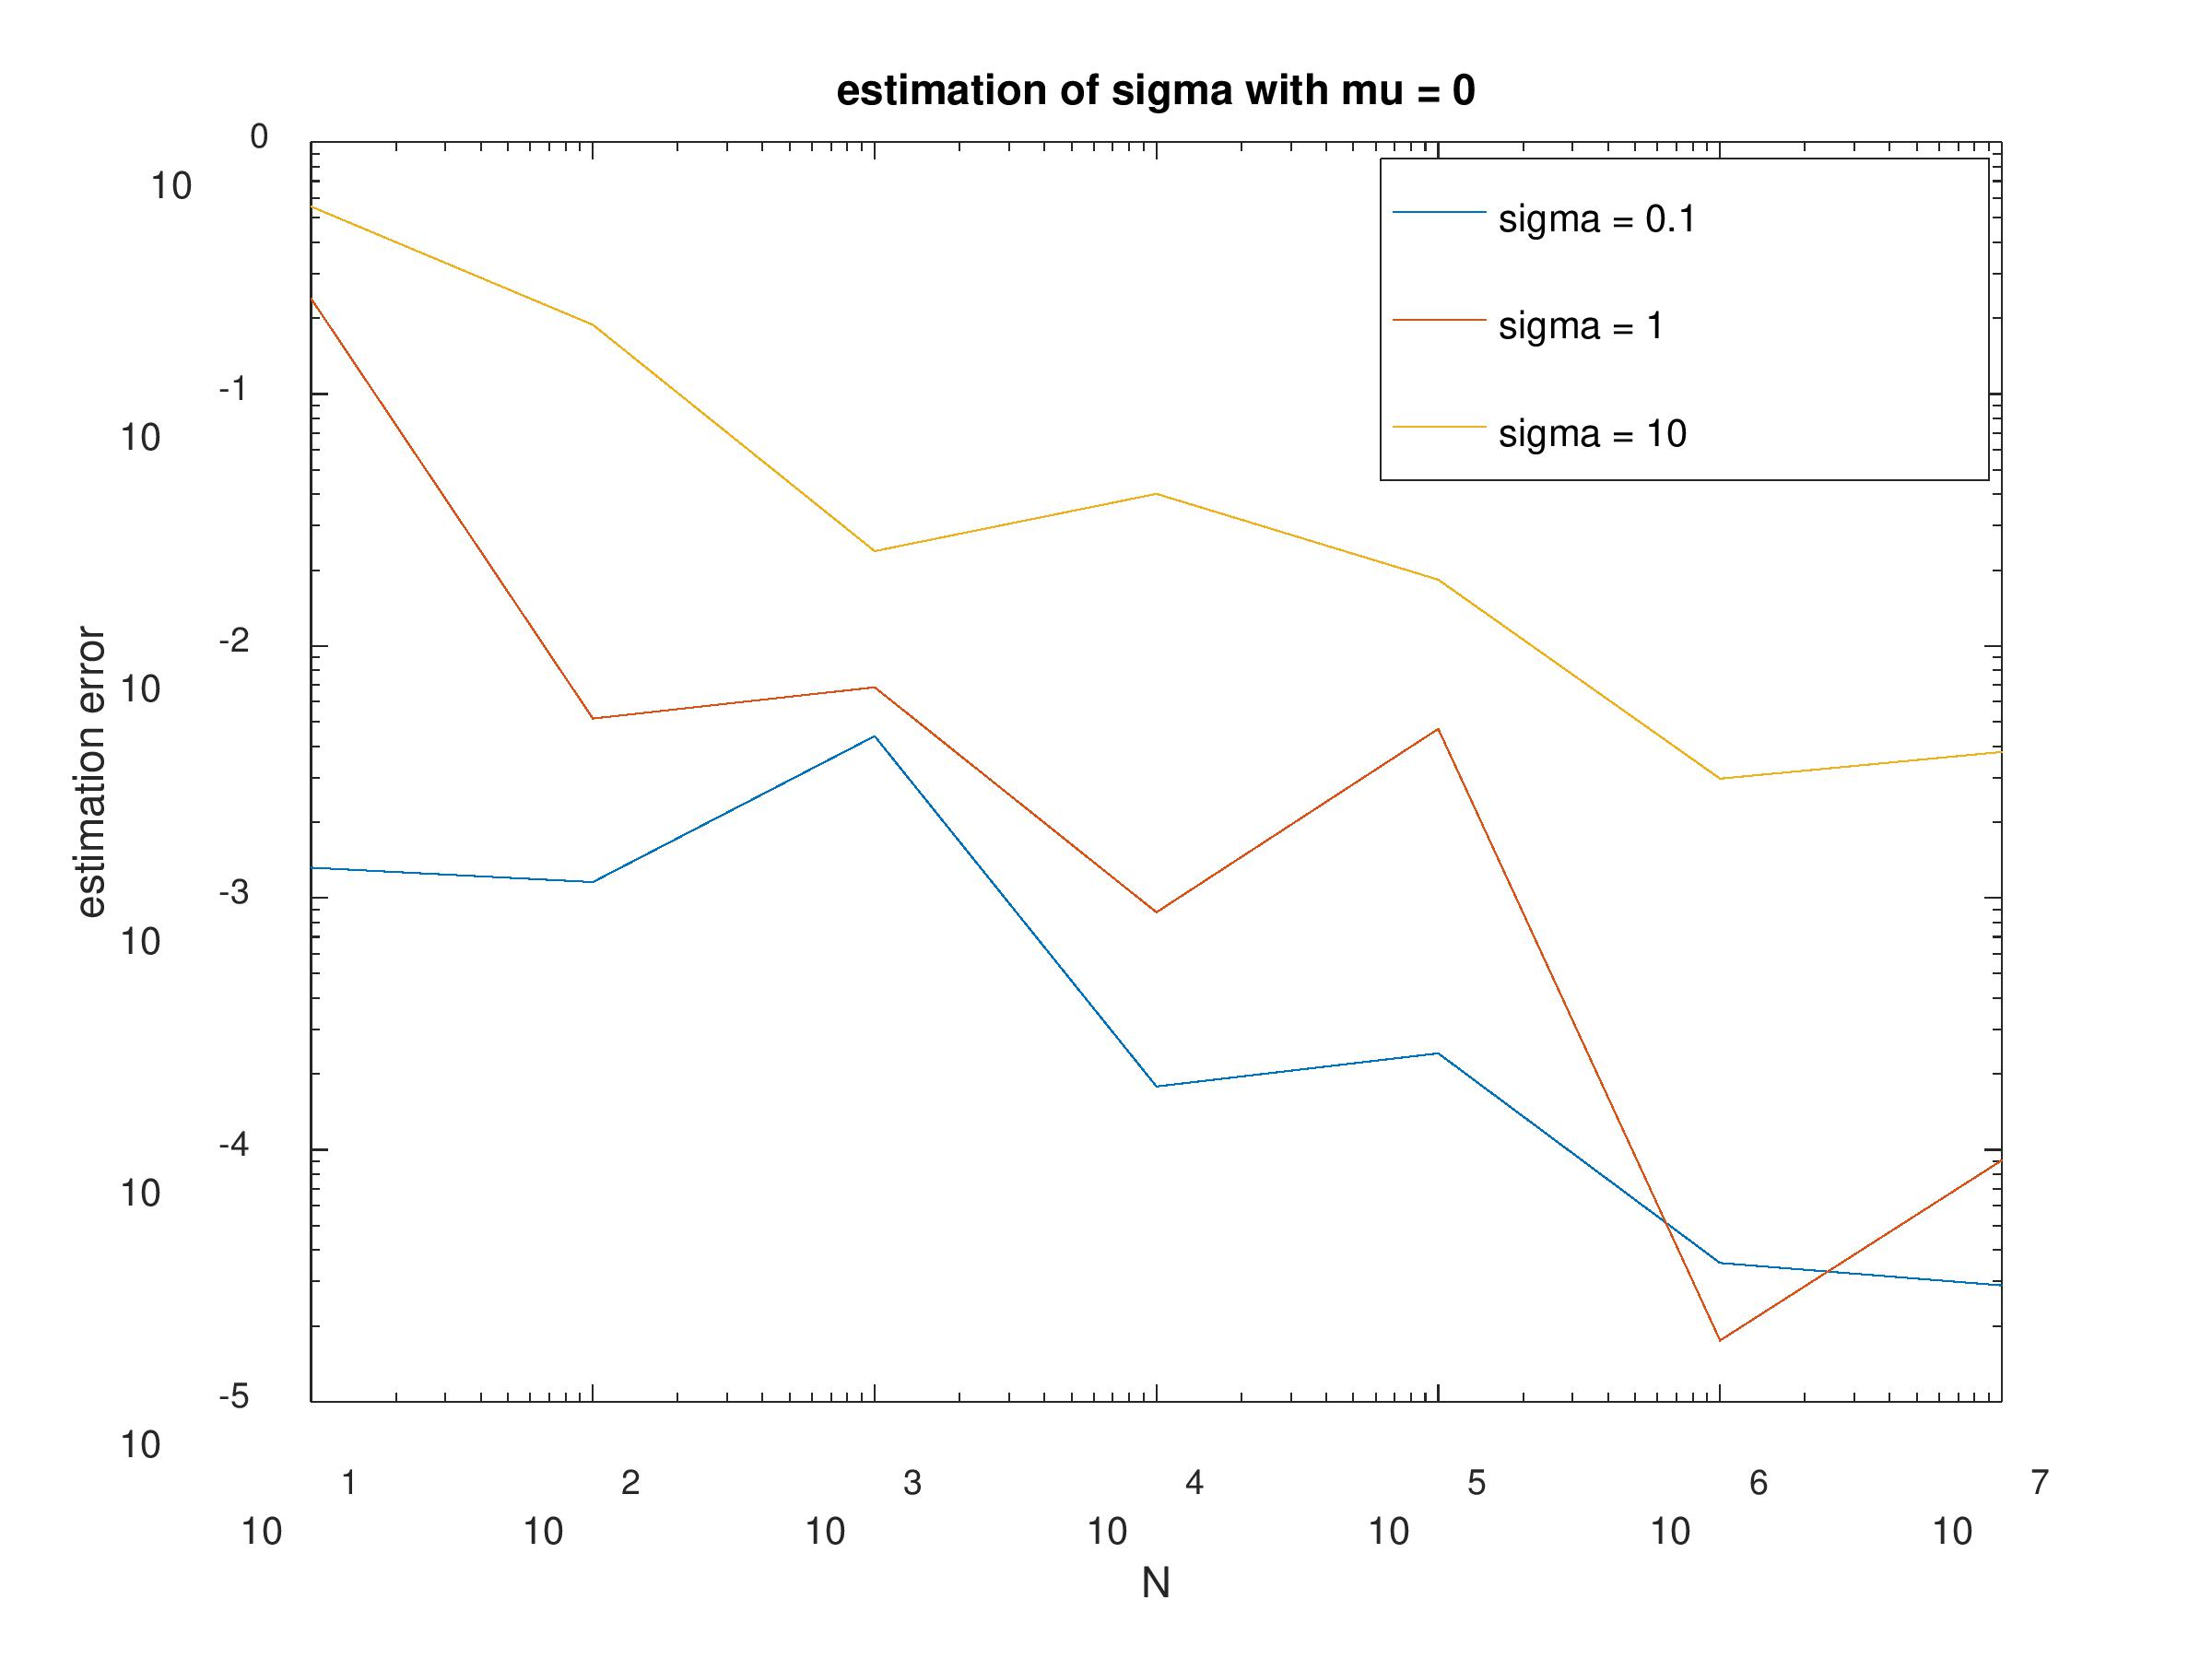
\includegraphics[scale=0.3]{sigma_err.jpeg}
\end{center}

\section*{Task 10}

\begin{center}
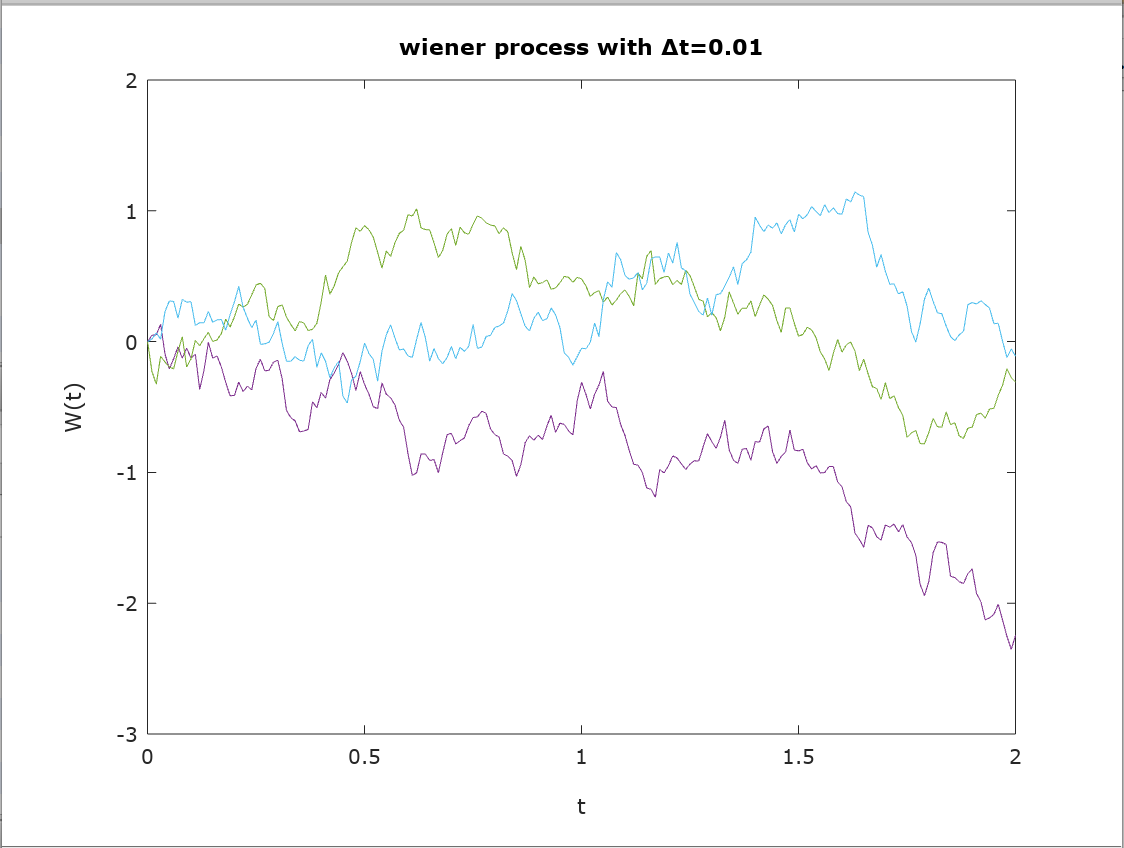
\includegraphics[scale=0.5]{wiener_001.jpeg}

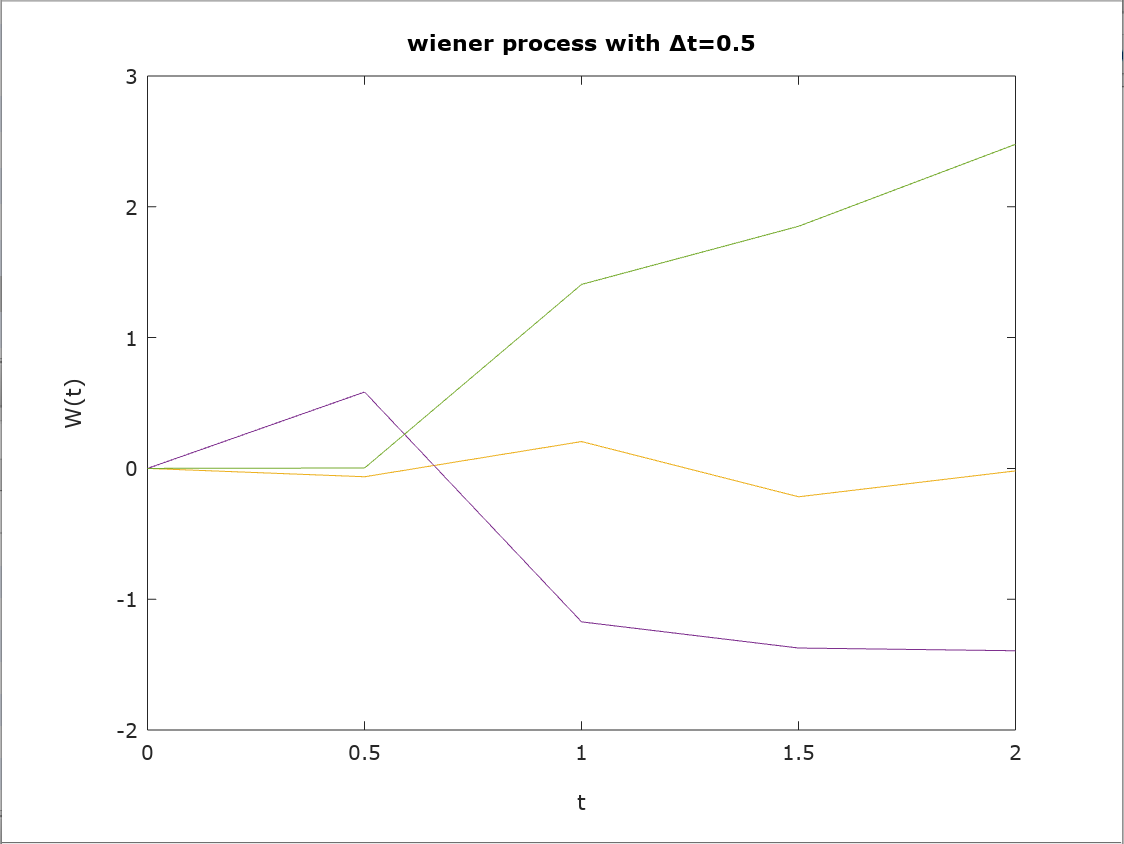
\includegraphics[scale=0.5]{wiener_05.jpeg}
\end{center}

\end{document}
